\documentclass[lettersize,journal]{IEEEtran}
\usepackage{amsmath,amsfonts}
\usepackage{algorithmic}
\usepackage{algorithm}
\usepackage{array}
\usepackage[caption=false,font=normalsize,labelfont=sf,textfont=sf]{subfig}
\usepackage{textcomp}
\usepackage{stfloats}
\usepackage{url}
\usepackage{verbatim}
\usepackage{graphicx}
\usepackage{cite}
%\usepackage[ruled, lined, linesnumbered, longend]{algorithm2e}
\hyphenation{op-tical net-works semi-conduc-tor IEEE-Xplore}
% updated with editorial comments 8/9/2021

\begin{document}

\title{Hardware Acceleration for BGV FHE using Prime-Factor FTT and Rader's Algorithm}

\author{David Du Pont, Jonas Bertels, Michiel Van Beirendonck, and Furkan Turan}

% The paper headers
%\markboth{IEEE JOURNALS}%
%{Shell \MakeLowercase{\textit{et al.}}: A Sample Article Using IEEEtran.cls for IEEE Journals}

%\IEEEpubid{0000--0000/00\$00.00~\copyright~2021 IEEE}
% Remember, if you use this you must call \IEEEpubidadjcol in the second
% column for its text to clear the IEEEpubid mark.

\maketitle

\begin{abstract}
Homomorphic Encryption enables computation on encrypted data, holding immense potential for enhancing data privacy and security in various applications. However, the adoption of fully homomorphic encryption schemes has been hindered by slow computation times. We presents a hardware architecture for efficient computation of the number theoretic transform within the context of fully homomorphic encryption using the BGV scheme. The architecture targets the specific parameter choice of the 21845-th cyclotomic polynomial, which is a practical parameter for BGV. The parameter 21845 also has ideal properties for use with the Prime-Factor FFT algorithm and Rader's algorithm. Using an efficient algorithm and leveraging parallel processing, pipelining and reuse of processing elements, the design achieves high throughput with optimized resource utilization. Simulation and implementation results on an Alveo U250 FPGA demonstrate the feasibility and performance of the proposed hardware design, making it a valuable contribution to the ongoing research and development efforts in the field of homomorphic encryption.
\end{abstract}

\begin{IEEEkeywords}
Fully Homomorphic Encryption, Harware Acceleration, Number Theoretic Transform, DoubleCRT.
\end{IEEEkeywords}

\section{Introduction}
\IEEEPARstart{I}{n} an era where data privacy and security have become important concerns, innovative cryptographic solutions are emerging to safeguard sensitive information while enabling efficient computations in untrusted environments. Among these advancements, Fully Homomorphic Encryption (FHE) stands out as a transformative technology that holds great promise across various sectors, including finance, web services, and beyond. FHE revolutionizes the paradigm of data processing by allowing computations to be performed directly on encrypted data, eliminating the risk of unauthorized access or the data being exposes in potential breaches.

In 2009, Craig Gentry's groundbreaking work introduced the first feasible construct for Fully Homomorphic Encryption, opening the door to a new realm of possibilities in secure computing \cite{10.1145/1536414.1536440}. Gentry's scheme allows both addition and multiplication operations, providing a foundation for constructing circuits that can perform arbitrary computations. Gentry started from a somewhat homomorphic encryption scheme and modified it so it can evaluate it's own decryption function and at least one more operation, a scheme like this is said to be bootstrappable. This operation of evaluating the decryption function homomorphically is very slow even on modern hardware. \cite{cryptoeprint:2014/873}

Smart and Vercauteren \cite{FHEsimd} observed that multiple plaintext values of a smaller ring can be packed into a single ciphertext. A single operation on this ciphertext corresponds to performing this operation on each of the plaintexts values individually in a SIMD fashion. This innovation lead to more efficient cryptosystems such as the BGV scheme \cite{BGV}. The operations in BGV are defined over a cyclotomic polynomial ring, therefore polynomial multiplication becomes the main performance bottleneck.

Open-source software library HElib\cite{helib} implements the BGV-FHE scheme with bootstrapping. HElib accelerates polynomial multiplication by using a different representation called DoubleCRT form. In DoubleCRT for polynomial multiplication become a simple pointwise multiplication of vector elements. To convert 

Halevi and Shoup \cite{cryptoeprint:2014/873} proposed an improved bootstrapping method for the BGV-FHE used in open-source software library HElib\cite{helib}.   Their method relies on having a polynomial ring of degree $m$ where $m$ has a special form. Practical values of $m$ are composed of few large prime factors. HElib accelerates polynomial multiplication by using a different representation called DoubleCRT form. In DoubleCRT form polynomial multiplication become a simple pointwise multiplication of vector elements. To convert between coefficient representation of a polynomial and DoubleCRT form a Number Theoretic Transform (NTT) is used. Many hardware architectures have been explored to accelerate the NTT operation for power-of-two values of $m$, but only few for non-power-of-two values.

In this paper we outline an hardware architecture, targeting HElib's BGV-FHE implementation for when the 21845-th cyclotomic polynomial is used. We use a combination of the Prime-Factor FFT algorithm and Rader's algorithm to reduce the arithmetic cost of the NTT computation. Circuit optimizations are used to achieve high performance. The two main techniques used are parallel processing to reduce the clock cycle count, and pipelining of the datapath to achieve a higher clock speed. An efficient memory design is used to keep up with the throughput. And we focus on maximal reuse of functional units throughout the different computation stages to keep the area or resource utilization on an FPGA limited. Finally, we compare our implementation to Wu et al.'s \cite{9937536} implementation of Bluestein's FFT.

\section{Preliminaries}
We use $\mathbb{Z}_q$ to denote the ring of integers with $q$ elements, also known as integers modulo $q$. In case $q$ is a prime number, $\mathbb{Z}_q$ forms a finite field. Elements in a ring are denoted by lowercase letters. Vectors of are expressed in bold $\mathbf{x} = \left \langle x_1, x_2, x_3, \ldots, x_{n-1}, x_n  \right \rangle$. The $i$-th component of vector $\mathbf{x}$ is specified as $x_i$. 

We use $\ast$ to represent the convolution operation between two vectors, whereas $\odot$ represents element wise multiplication. 

\subsection{The BGV Scheme}
The BGV scheme operates on polynomials over cyclotomic rings. The plaintext space of the BGV scheme consists of vectors of integers modulo a plaintext modulus. The ciphertext space of the BGV scheme consists of vectors of polynomials modulo a ciphertext modulus, which is a large integer that determines the security level and the noise budget. An important feature of the BGV scheme is the concept of modulus switching. A freshly encrypted ciphertext starts at encryption level $L$ and the encryption level gradually moves down as we perform homomorphic computations. With each encryption level $l$ a modulus $q_l$ is associated. Modulus switching helps to reduce the noise growth because when we switch the modulus from $q_l$ to $q_{l-1}$ with $q_{l-1} > q_l$ the noise term of the ciphertext is reduced by the ratio $\frac{q_l}{q_{l-1}}$. When we reach the smallest modulus $q_0$ at encryption level 0, the noise can no longer be reduced. At this point the ciphertexts needs to either be decrypted or Gentry's bootstrapping method\cite{10.1145/1536414.1536440} needs to be employed to enable further computation.

In the implementation of the BGV scheme within HElib, a series of small machine-word sized prime numbers ${p_0, p_1, p_2, \ldots, p_L}$ are used to construct moduli as follows:\cite{cryptoeprint:2014/873} 

\begin{equation}
q_l = \prod_{i=0}^{i=l} p_i
\end{equation}

The BGV scheme involves various operations with integer polynomials, such as modular multiplications, additions, and Frobenius maps. To increase efficiency, the polynomials used in these operations are represented using the DoubleCRT format. This format represents a polynomial as a collection of polynomials, each computed modulo a small primes $p_l$, with each individual polynomial further represented in evaluation form. In this evaluation form, a polynomial is described as a vector containing its values at primitive $N$-th roots of unity within the finite field $\mathbb{Z}_{p_l}$. Using this representation, polynomial multiplication simplifies to pointwise multiplication that can be performed in linear time. The transformation between coefficient representation, where the polynomial is expressed as a list of its coefficients, and evaluation representation involves using the Number Theoretic Transform (NTT). The NTT happens to be the most time-consuming step for calculations in HElib, therefore it is the primary focus of hardware acceleration.

\subsection{Bootstrappable Parameters for HElib}
HElib utilizes Smart and Vercauteren's technique\cite{FHEsimd} for efficient SIMD operations on encrypted data by packing multiple values into a single plaintext. The algorithms HElib uses to make this possible impose strong restrictions on the parameter $m$, which denotes the number of coefficients in the plaintext polynomial. This causes useful values of $m$ to have few divisors. Halevi and Shoup\cite{cryptoeprint:2014/873} used a brute force search method to identify useful values for $m$. Notably $m=21845$ and $m=65535$ are optimal choices for the prime-factor FFT algorithm and Rader's algorithm due to their prime factors being of the form $2^n + 1$.

\subsection{Number Theoretic Transform (NTT)}
The number theoretic transform (NTT) generalizes the discrete Fourier transform (DFT) over $\mathbb{Z}_p$ where $p$ is prime.
It provides efficient algorithms for polynomial multiplication. \cite{cryptoeprint:2016/504}
$\mathbb{Z}_p$ is a finite field, so there exists a primitive $N$-th root of unity if $N$ divides $p-1$.
Let $\omega$ be a primitive $N$-th root of unity then the N-point NTT $\mathbf{X}=\mathcal{N}\left\{\mathbf{x}\right\}$ is defined as:

\begin{equation}
X_k = \sum_{n=0}^{N-1} x_n \omega^{nk} \qquad k=0,\ldots,N-1
\end{equation}

The inverse NTT $\mathbf{x}=\mathcal{N}^{-1}\left(\mathbf{X}\right)$ is defined as:

\begin{equation}
x_n = N^{-1}\sum_{k=0}^{N-1} X_k \omega^{-nk} \qquad k=0,\ldots,N-1
\end{equation}

Since $\omega$ is an N-th root of unity we have $\omega^{-nk} = \omega^{(N-k)n}$. This means an inverse NTT can be computed using a forward NTT by reversing the order of the elements in $\mathbf{X}$ as follows:

\begin{equation}
\label{eq:reverse_order}
\left \langle X_0, X_{N-1}, X_{N-2}, \ldots, X_2, X_1 \right \rangle
\end{equation}

Because of the similarity between the NTT and DFT, any FFT algortihm can also be used for calculating the NTT.
The only modification that needs to be made is that $e^{-\frac{j2\pi}{N}}$ is replaced by $\omega$. \cite{1162555}

\subsection{Prime-Factor FFT Algorithm}
The prime factor FFT algorithm (PFA) re-expresses a discrete Fourier transformation (DFT) of size $N = N_1 N_2$ as a two-dimensional $N_1 \times N_2$ DFT. \cite{1671829} $N_1$ and $N_2$ should be coprime integers. The smaller transforms of size $N_1$ and $N_2$ can be evaluated by applying PFA recursively, or by using another FFT algorithm. The factorization is similar to Cooley-Tukey but has the advantage that no multiplications with twiddle factors are required. However, its use is limited to coprime factorizations, and a more complex re-indexing based on the Chinese remainder theorem (CRT) is required.

\subsection{Rader's Algorithm}
Rader's algorithm permits to efficiently compute the N-point NTT when $N$ is prime. \cite{1448407} In $\mathbb{Z}_N$, there exists a primitive root $g \in \mathbb{Z}_N$ such that for any non-zero element $n \in \mathbb{Z}_N$, there exists a unique exponent $q \in \{0, 1, 2, \ldots, N-2\}$ satisfying the equation: $n = g^q \pmod{N}$. Since every non-zero element in $\mathbb{Z}_N$ corresponds to a unique $q$ this forms a bijection from $q$ to non-zero $n$. In the same way $k = g^{-p} \pmod{N}$, with k a non-zero element in $\mathbb{Z}_N$ and $p \in \{0, 1, 2, \ldots, m-2\}$ forms a bijection from $p$ to non-zero $k$. By using this re-indexing the NTT can be expressed as the convolution of two sequences $\mathbf{a}$ and $\mathbf{b}$ as follows:

%\begin{equation}
%\begin{split}
\begin{align}
a_q &= x_{g^q} \\
b_q &= \omega^{g^{-q}} \\
X_{g^{-p}} &= x_0 + \sum_{n=0}^{N-2} a_q b_{p-q} \qquad p=0,\ldots,N-2
\end{align}
%\end{split}
%\end{equation}

The convolution is computed by using the convolution theorem (\ref{eq:conv_theorem}).

\begin{equation}
\label{eq:conv_theorem}
\mathbf{a} \ast \mathbf{b} = \mathcal{N}^{-1}\left\{\mathbf{A}\odot \mathbf{B}\right\}
\end{equation}

Rader's algorithm requires $m-1$ additions to compute $X_0 = \sum_{i=0}^{m-1} x_i$ and $m-1$ additions to add $x_0$ to each element of the convolution result. This number can be reduced to just two additions. We observe that

\begin{equation}
A_0 = \sum_{q=0}^{N-2} x_{g^q} = \sum_{i=1}^{N-1} x_i
\end{equation}

so $X_0$ can be computed as $X_0 = x_0 + A_0$. If $\mathbf{C} = \mathbf{A} \odot \mathbf{B}$, then adding $x_0$ to $C_0$ before the inverse NTT corresponds to adding $x_0$ to each element of $\mathbf{c}$. Algorithm \ref{alg:rader} describes our implementation of Rader's algorithm with these modifications. Note that we exclude the final reversed re-indexing step.

\begin{algorithm}[H]
\caption{Optimized Rader's Algorithm}\label{alg:rader}
\begin{algorithmic}
\STATE 
\STATE {\textsc{RADER}}$(\mathbf{x})$
\STATE \hspace{0.5cm}$ \mathbf{x^\prime} \gets$ {\textbf{RaderPermutation}}$([x_1, x_2,\ldots, x_{m-1}]) $
\STATE \hspace{0.5cm}$ \mathbf{A} \gets \mathcal{N}(\mathbf{x^\prime}) $
\STATE \hspace{0.5cm}$ X_0 \gets A_0 + x_0 $
\STATE \hspace{0.5cm}$ \mathbf{C} \gets \mathbf{B} \odot \mathbf{A} $
\STATE \hspace{0.5cm}$ C_0 \gets C_0 + x_0 $
\STATE \hspace{0.5cm}$[X_1, X_2,\ldots, X_{m-1}] \gets \mathcal{N}^{-1}\left(\mathbf{C}\right)$
\STATE \hspace{0.5cm}\textbf{return}  $\mathbf{X}$
\STATE 
\end{algorithmic}
\end{algorithm}

\section{Hardware Implementation}
The architecture is designed for the 21845-th cyclotomic polynomial, which is a practical parameter to use in BGV-FHE. \cite{cryptoeprint:2014/873} The NTT circuit can work with up to 46 different moduli of 32 bits, this is necessary for modulus switching in the BGV scheme. Only forward NTTs are supported, but an inverse NTT can be computed by performing a re-indexing in software that puts the elements in the order as shown in (\ref{eq:reverse_order}). 

\subsection{Overview}

Figure \ref{fig:hardware_overview} shows an overview of the hardware architecture. The hardware exploits data parallelism by performing operations on large vectors. The data is streamed through a fully pipelined datapath. Given that the processor is pipelined, a high clock rate can be applied. And since there are no wait states, all processing elements are optimally used. This result is a very efficient implementation.

Vectors are composed of 257 32-bit words. 257 corresponds to the largest dimension in the resulting $257 \times 85$ matrix obtained through PFA. Each vector can represent either one row of the matrix or three columns. As the vectors pass through the datapad, either one recursive stage of the Cooley-Tukey FFT algorithm or 128 pointwise multiplications can be computed. Each functional unit in the architecture is designed to handle a throughput of one vector per cycle. The NTT unit consists of 128 radix-2 butterfly units. These units can be configured to perform either a butterfly operation or only a multiplication and modular reduction.

To achieve the required memory bandwidth, we use 257 individually addressable memory banks. The rows of the matrix are stored in a staggered manner, ensuring that each element of a row or column resides in a different memory bank. An address generator determines the read and write addresses, while barrel shifters eliminate and reapply the offset caused by row staggering.

\begin{figure}[h]
\centering
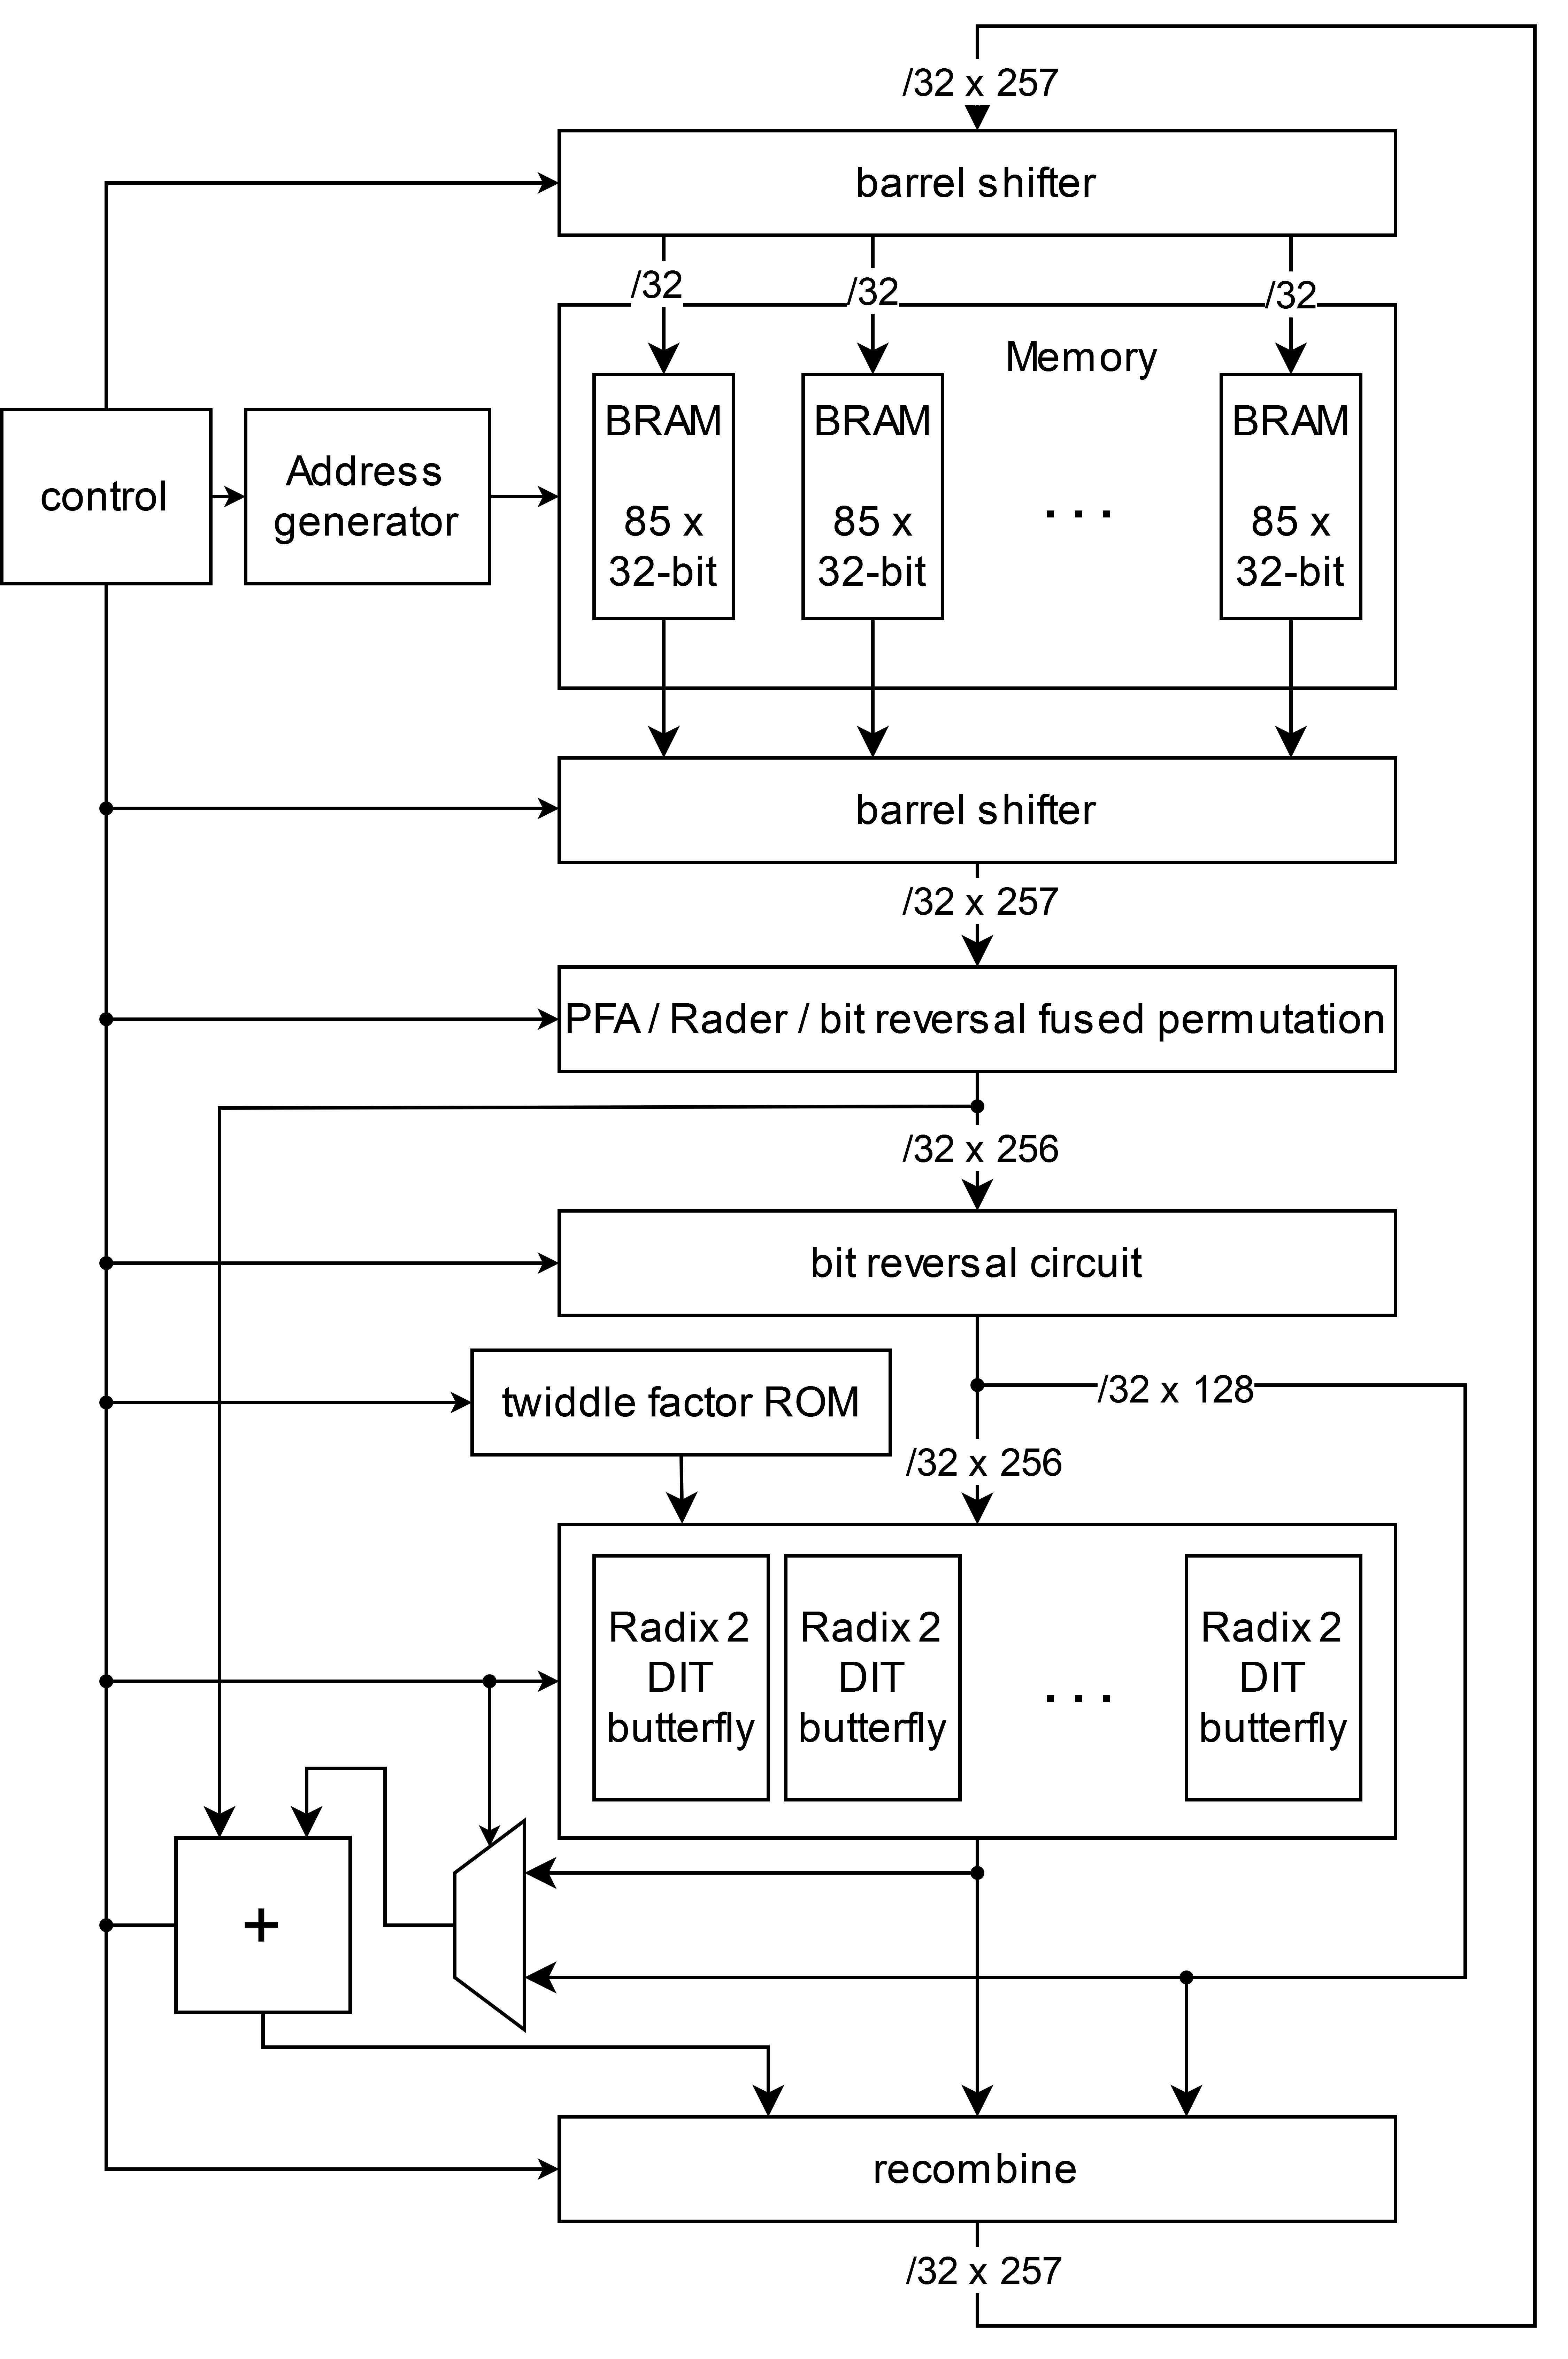
\includegraphics[width=2.5in]{img/architecture.png}
\caption{Proposed FFT hardware architecture}
\label{fig:hardware_overview}
\end{figure}

\subsection{Control Flow}
Figure \ref{fig:state_diagram} illustrates the state diagram of the controller, which governs the processing of a three-dimensional grid with dimensions $257 \times 17 \times 5$ obtained through PFA. The outer loop in the controller contains seven distinct states, including the initial idle state. Additionaly, three state variables are present: \emph{axis}, \emph{row} and \emph{step}. \emph{axis} indicates the traversal direction within the grid, \emph{row} indicates the currently processed row index, and \emph{step} corresponds to the Cooley-Tukey algorithm stage. The output of the controller depends on both the current state and the current axis.

Each stage of the NTT computation is performed on all rows along one axis before moving on to the next stage. Iterating over the NTT stages in the outer loop and over the rows in the inner loop eliminates data dependencies that would cause pipeline stalls. The iteration order is different for the Multiply part 1 and Multiply part 2 states which encompass the point-wise multiplication in Rader's algorithm \ref{alg:rader}. Iterating over the rows in the outer loop is more efficient for these operations since there is no data dependency. Moreover, some of the data required for part 2 would be overwritten by the result of part 1, this is avoided by performing both operations for the same row in subsequent cycles.

The pipeline stalls in the final state, where we wait for all NTTs along the current axis to complete. This stalling is necessary when transitioning from rows to columns because there is a data dependency between each row and column.

\begin{figure}[h]
\centering
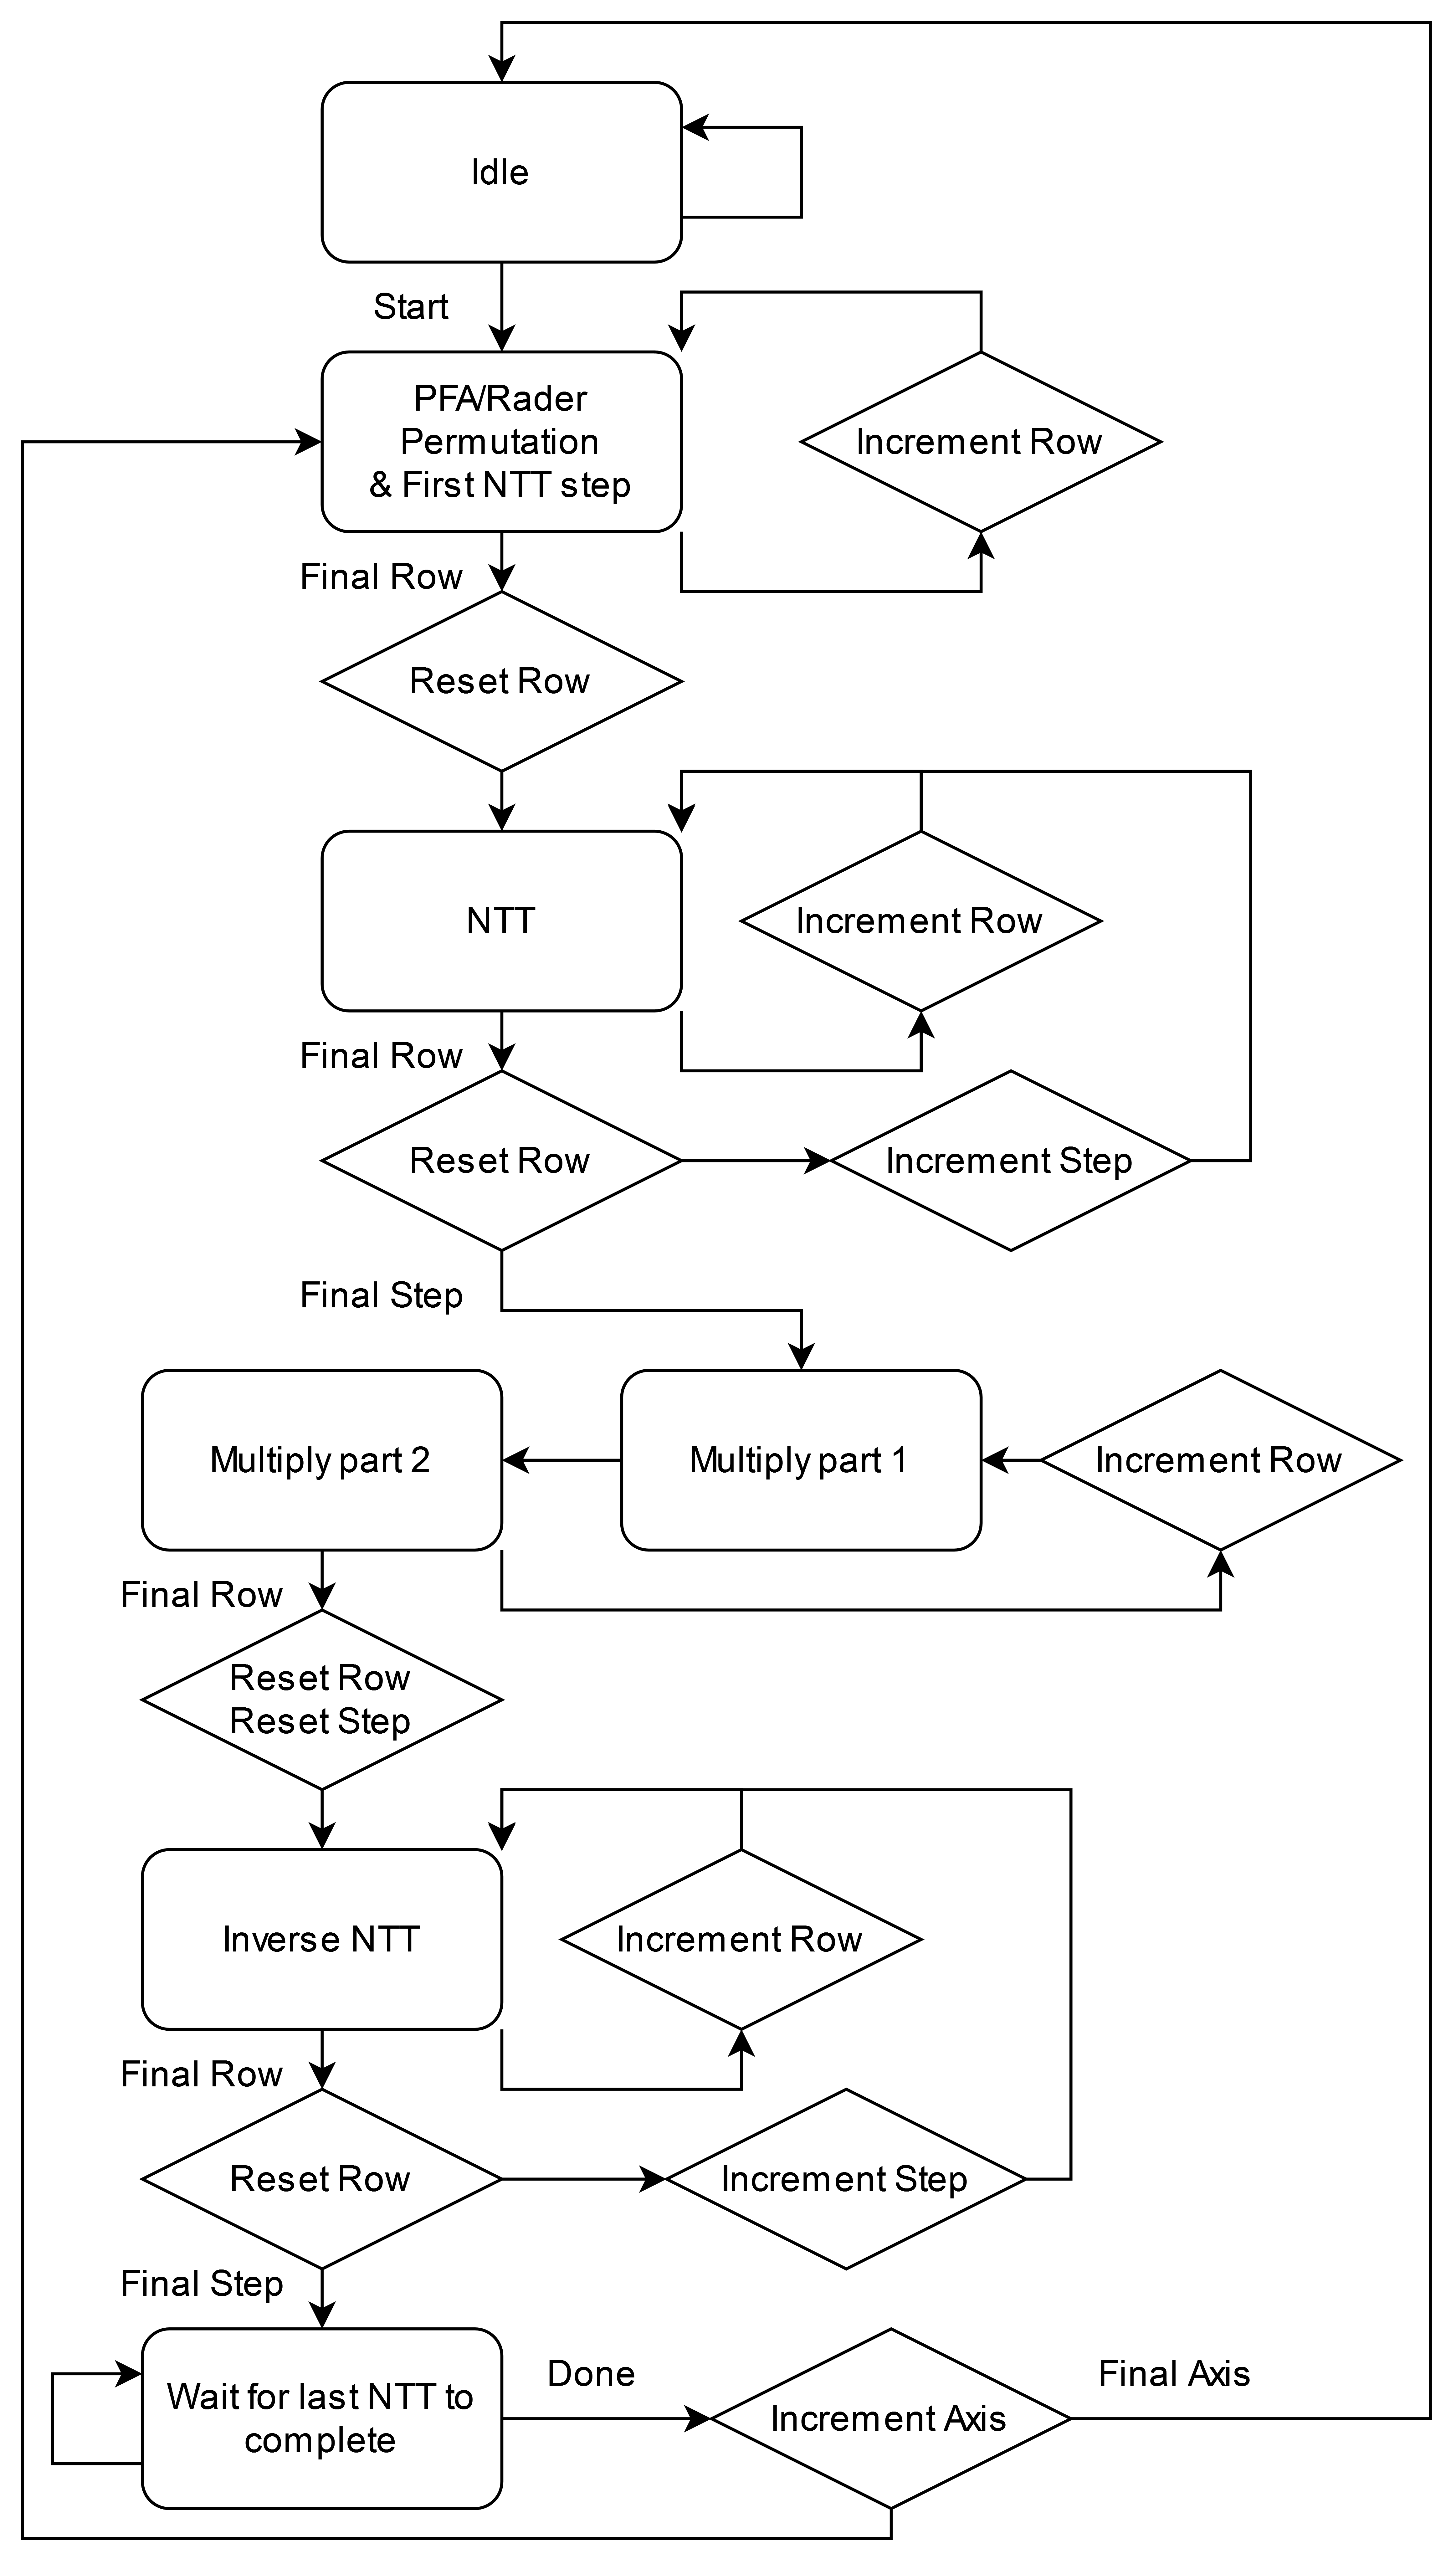
\includegraphics[width=2.5in]{img/control_flow.png}
\caption{Control state diagram}
\label{fig:state_diagram}
\end{figure}

\subsection{Memory Design}
PFA re-expresses the NTT of size $m = 21845$ as a two-dimensional NTT over a $257\times 85$ matrix. This matrix is stored in 257 Block RAMs (BRAM) on the FPGA so that a vector of 257 32-bit words can be read from or written to the memory in every cycle.

Accessing matrix elements in parallel poses a challenge. Namely, storing columns in separate BRAMs enables parallel row access but not parallel column access, while storing rows in separate BRAMs enables parallel column access but not parallel row access. To address this, a staggered memory arrangement is used. Rows are stored offset by one BRAM from each other, enabling parallel access to both rows and columns. See Figure \ref{fig:staggered_memory} for a visual example using a 7×5 matrix. Each color corresponds to a distinct matrix column, highlighting separate BRAM storage for both rows and column elements.

\begin{figure}[H]
\centering
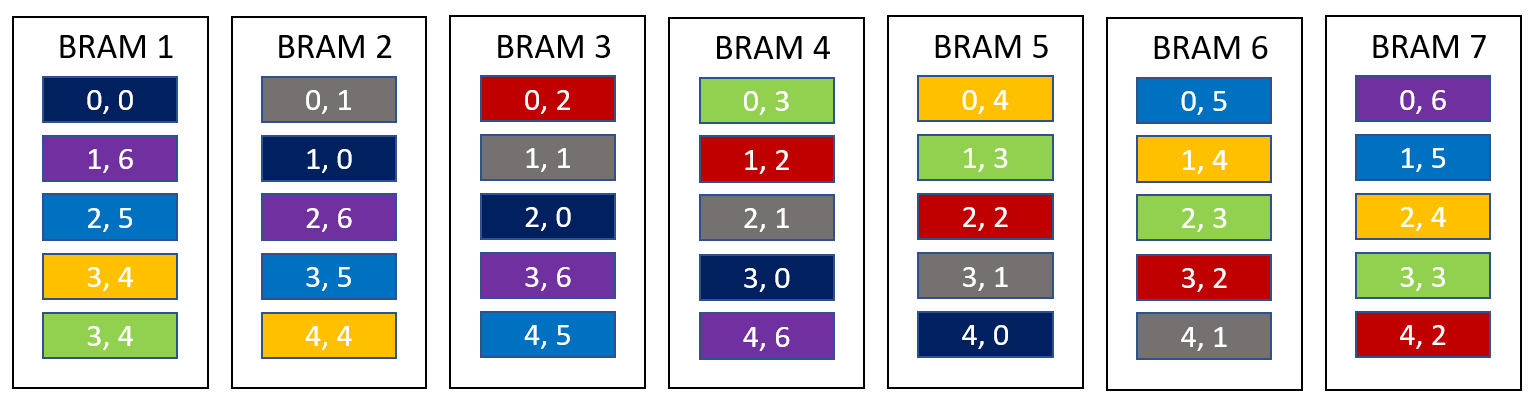
\includegraphics[width=3.5in]{img/staggered_memory.png}
\caption{Illustration of staggered rows in memory, each color represents a column in the PFA matrix.}
\label{fig:staggered_memory}
\end{figure}

To facilitate reading from and writing to memory with the required offsets, two circular shift circuits are needed: one at the write ports and another at the read ports of the memory. These circuits enable circularly shifting 32-bit words across lanes in a vector of length 257. A barrel shifter is used to achieve a throughput of one vector per cycle.

\subsection{Combining Permutations}
The NTTs of size 85 over the columns are re-expressed as a two-dimensional NTT over a $17\times 5$ matrix. This translates to two two distinct permutations in our hardware: one that groups the elements of every matrix row together and one that groups the columns of the matrix instead.

The NTTs of size 257, 17 and 5 are computed using Rader's algorithm. In Rader's algorithm, the first element of each row (with sizes 257, 17, and 5) in the vector needs to be removed. A permutation removes the first points from the NTT vectors and fills the gaps with subsequent elements. The removed first points are collected and placed at the end of the vector. An additional permutation is required for the re-indexing in Rader's algorithm. This permutation is different for each NTT size (257, 17, and 5).

Furthermore, a bit-reversal permutation is necessary because the decimation in time Cooley-Tukey algorithm expects the initial input in a bit-reversed order.

It seems that there are many permutations involved, but by combining certain permutations, their total number can be reduced to six. To select one permutation from the reduced set of six, a 6-to-1 multiplexers are used.

\subsection{Vectorized Cooley-Tukey FFT}
The radix-2 decimation-in-time (DIT) Cooley–Tukey FFT algorithm, recursively breaks down a DFT of composite size $2n$ into $2$ smaller transforms of size $n$. These smaller DFTs are then combined via size-2 butterflies, which themselves are DFTs of size 2 premultiplied with roots of unity known as twiddle factors. Figure Figure \ref{fig:dit_fft} shows a butterfly diagram for an 8-point FFT algorithm, which illustrates how the inputs and outputs are connected for each stage during the computation. The same hardware used for computing an FFT of size $2n$ can also be used for computing two FFTs of size $n$ by omitting the final stage of the FFT and adjusting the twiddle factors. This property allows us to reuse the hardware of a 256-point FFT, for computing multiple 16-point and 4-point FFTs in parallel.

\begin{figure}[h]
\centering
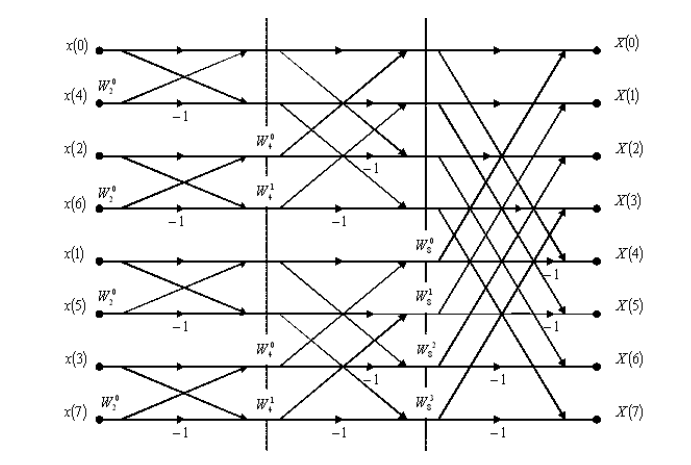
\includegraphics[width=2.5in]{img/dit_fft.png}
\caption{Butterfly diagram for radix-2 DIT FFT algorithm from Pace et al. \cite{ditfftimg}}
\label{fig:dit_fft}
\end{figure}

The bit-reversal circuit is very simple. To achieve a throughput of one vector per cycle, it is implemented as a series of eight bit-reversal permutations of increasing length $\{2, 4, 8, 16, 32, 64, 128, 256\}$. Multiplexers are used to select either the permuted vector or the non-permuted vector.

\subsection{Butterfly Units}

We uses 128 butterfly units to achieve a throughput of one vector per cycle. The design of a butterfly unit is depicted in Figure \ref{fig:dit_rader_butterfly}.

\begin{figure}[h]
\centering
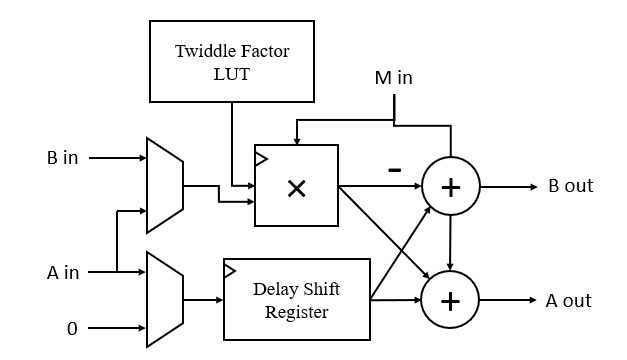
\includegraphics[width=2.5in]{img/dit_rader_butterfly.png}
\caption{Implementation of radix-2 DIT FFT butterfly}
\label{fig:dit_rader_butterfly}
\end{figure}

The butterfly unit makes use of a word-level Montgomery modular multiplier implementation from Mert et al. \cite{9171507}. The multiplier is fully pipelined and has a latency of eleven cycles. A shift register is used to match the latency of the modular multiplier for the other input. Twiddle factors are precomputed and stored in a lookup table.

The convolution in Rader's algorithm requires a pointwise product to be computed. To optimize resource utilization, we repurpose existing butterfly unit multipliers for this task. One of the factors in each pointwise product is a precomputed constant, conveniently stored within the FFT twiddle factor lookup table. To perform multiplication without the final addition, we add a multiplexer at input A that allows a zero input selection. Another multiplexer is added at input B to enable multiplication of either input A or input B with a constant factor.

\section{Results}

\subsection{Simulation Results}

Verilog simulation involves writing data into the BRAMs from a file, followed by the full NTT computation. The simulation showed that a 21845-point NTT can be computed in 2957 clock cycles. This number is consistent regardless of the data or modulus used. 2392 clock cycles are spent in computing the FFTs using Cooley-Tukey's algorithm, 514 clock cycles in pointwise multiplication for Rader's algorithm and 51 cycles are pipeline stalls which corresponds to only 1.7\% of the total execution time.

\subsection{Implementation Results}

The implementation results are shown in Table \ref{table:implementation_results}. These results include the entire NTT but without BRAM interface. 257 of the BRAMs are used as RAM, and 171 BRAMs are used as ROM to store the twiddle factors. The Alveo u250 FPGA contains BRAM tiles which can implement either one large BRAM or two smaller BRAMs. The ROM BRAMs use one tile each, the RAM BRAMs use 128.5 tiles. Therefore utilization reports show 299.5 BRAMs used.

The implementation run with default settings in Vivado suffered from SLL (Super Long Line) congestion. SLLs connect signals between large regions called Super Logic Regions (SLR) on the FPGA. There are only a limited number of these connections available and the router has difficulty with timing closure when a high portion of these SLLs is used. To address this problem the placer directive SSI\_BalanceSLLs was used which eliminated the use of SLLs entirely by confining all the logic to one SLR. The single SLR placement solves the SLL congestion but introduced routing congestion on the connections within the SLR, therefore the clock frequency had to be lowered from 200 MHz in synthesis to 125 MHz after placement.

\begin{table}[h]
\centering
\begin{tabular}{ *{5}{|c}| } 
 \hline
 Frequency (MHz) &  CLB LUT & CLB Register & BRAM  & DSP  \\ \hline
 125             &  230043  & 118765       & 299.5 & 1024 \\
 \hline
\end{tabular}
\caption{Implementation results}
\label{table:implementation_results}
\end{table}


\subsection{Comparison to Other Implementations}
Few efforts have been made in hardware acceleration of NTTs with non-power-of-two lengths. Wu et al. \cite{9937536} uses Bluestein's algorithm. To the best of our knowledge, this is the only non-power-of-two implementation of comparable size. Their implementation can not be used for BGV-FHE in the same way since it supports only a single modulus. Despite this we will focus mostly on on Wu et al.'s implementation, since the other implementations are only suitable for power-of-two length NTTs. \cite{ozturk2574340, 10.1145/3373376.3378523, 9171507, cryptoeprint:2013/866, cryptoeprint:2020/446}

To facilitate performance comparison, Table \ref{table:implementation_comparison} presents the cycle count for one forward NTT computation normalized to $m=1024$ and $k=32$, where $k$ is the modulus size in bits. We assume quasilinear scaling with $m$ due to the FFT operation's time complexity. Linear performance scaling is assumed for $k$ as lowering the small moduli's bit-width in the BGV scheme roughly corresponds to a proportional increase in the number of vectors in DoubleCRT representation. The normalized cycle count $\tilde{c}$ is calculated as

\begin{equation}
\label{eq:norm_cycles}
\tilde{c}=\text{cycles}\cdot\frac{32 \cdot 1024 \log_2 1024}{k \cdot m \log_2 m}
\end{equation}

The table also includes the products of the normalized cycle count with the number of LUTs and DSPs, indicating better performance with lower values. It's important to note that this performance estimation does not consider other potential limitations.

Wu et al.'s implementation performs better on this metric when a 8193-point NTT is considered, which would be the best case for their implementation. A more practical parameter for BGV would be $m=4369$. \cite{9937536} In this case our design performs significantly better. It is important to note that Wu et al.'s design makes use of a specific modulus to greatly simplify modular reduction, using the technique would result in a 50\% decrease in DSPs for our design. Our design does not incorporate hardware-based reversed re-indexing, resulting in a scrambled NTT result. This reversed re-indexing step can be performed in linear time and is not necessary for element-wise operations, but is required when we convert back from DoubleCRT to polynomial coefficient representation.

\begin{table*}[!t]
\caption{Comparison to other implementation results.}
\label{table:implementation_comparison}
\centering
\begin{tabular}{ |l*{7}{|m{0.09\textwidth}}| } 
 \hline
 Design               & This work   & Wu et al.\cite{9937536} & \cite{ozturk2574340} & \cite{10.1145/3373376.3378523} & \cite{9171507} & \cite{cryptoeprint:2013/866} & \cite{cryptoeprint:2020/446} \\ \hline \hline
 $m$                  & 21845       & 8193 / 4369  & 32768    & 8192                & 4096     & 512      & 1024      \\  \hline
 Modulus size (bits)  & 32          & 64           & 32       & 54                  & 60       & 13       & 16        \\  \hline
 Platform             & Alveo U250  & Virtex-7     & Virtex-7 & Stratix 10 GX 2800  & Virtex-7 & Virtex 6 & Arktix-7  \\  \hline
 Frequency (MHz)      & 125         & 250          & 250      & 300                 & 125      & 278      & 45.47     \\  \hline
 Cycles               & 2957        & 5825         & 12725    & 768                 & 972      & 2304     & 18537     \\  \hline
 CLB LUTs             & 230k        & 76.2k        & 219k     & 142k                & 99.3k    & 1536     & 2908      \\  \hline
 CLB Registers        & 118k        & -            & 90.7k    & 387k                & -        & 953      & 170       \\  \hline
 BRAM                 & 428         & 62           & 193      & 725                 & 176      & 3        & 0         \\  \hline
 DSPs                 & 1024        & 256          & 768      & 320                 & 929      & 1        & 9         \\  \hline
 $\tilde{c}$          & 96.1        & 280 / 565    & 265      & 73.8                & 203      & 7651     & 18537     \\  \hline
 $\tilde{c}$ $\times$ LUTs& 22\,116\,274 & 21\,339\,663 / 43\,013\,187 & 58\,057\,813 & 6\,214\,017 & 10\,724\,400 & 19\,358\,326 & 107\,811\,192 \\ \hline
 $\tilde{c}$ $\times$ DSPs& 98\,465      & 71\,692 / 144\,506 & 203\,600 & 14\,003 & 100\,332 & 12\,603 & 333\,666 \\
 \hline
\end{tabular}
\end{table*}

\section{Conclusion}
In this work, we presented a hardware architecture for efficient non-power-of-two number theoretic transform computations, targeting fully homomorphic encryption using the BGV scheme. Our design focuses on the 21845-th cyclotomic polynomial, which is a practical parameter for BGV. We used efficient arithmetic
and algorithmic optimization techniques and leveraged parallel processing, pipelining, and optimized memory management to achieve high performance. The simulation and implementation results have demonstrated its competitive performance as compared to existing implementations for both power-of-two and non-power-of-two NTT sizes.

 % argument is your BibTeX string definitions and bibliography database(s)
\bibliography{references}
%
\bibliographystyle{IEEEtran}


\newpage

 
\vfill

\end{document}


